\chapter{Resultados preliminares e discussão}
\label{cap:resultados}

Este capítulo apresenta duas avaliações complementares. A primeira compara as previsões automáticas com as anotações do autor em cem notícias sobre a Sabesp. A segunda investiga como o ITI, construído com a representação contextual das notícias, se associa aos retornos posteriores da ação SBSP3. A distinção é necessária porque as duas avaliações utilizam entradas textuais diferentes. Os resultados são discutidos separadamente antes de examinar suas implicações conjuntas.

\section{Avaliação do sinal textual}

\subsection{Rodadas de anotação e concordância com o classificador}

As cem notícias da avaliação textual foram anotadas pelo autor conforme o protocolo orientado ao efeito para a Sabesp, datado de 7 de outubro de 2026. Uma rodada anterior utilizou critérios mais simples e produziu acurácia de 48\% e kappa de 0,163. Como a definição da tarefa foi alterada entre as rodadas, esses valores não representam uma trajetória comparável de melhora ou piora do classificador.

Na avaliação utilizada nesta qualificação, o FinBERT-PT-BR concordou com o autor em cinquenta das cem notícias. A acurácia de 50\% precisa ser considerada junto à composição da referência: 67 matérias receberam o rótulo neutro. Uma regra que atribuísse ``neutro'' a todos os textos alcançaria 67\% de acurácia, embora não reconhecesse nenhum exemplo positivo ou negativo. A comparação demonstra que a acurácia isolada não é suficiente para julgar a qualidade das previsões. O F1 macro de 0,45 e o kappa de Cohen de 0,197 complementam essa avaliação, sem substituir a inspeção dos erros por classe.

\begin{table}[htbp]
\centering
\caption{Concordância do FinBERT-PT-BR com as anotações do autor, em 100 notícias sobre a Sabesp.}
\label{tab:avaliacao-texto}
\begin{tabularx}{\textwidth}{@{}Lrrrr@{}}
\toprule
Subconjunto & $n$ & Acurácia & Kappa & F1 macro \\
\midrule
Amostra completa & 100 & 50,0\% & 0,197 & 0,45 \\
Matérias focais & 74 & 52,7\% & $\simeq 0{,}26$ & --- \\
Agenda ou multiempresa & 26 & 42,3\% & $\simeq -0{,}03$ & --- \\
\bottomrule
\end{tabularx}
\vspace{0.4em}
{\footnotesize Fonte: resultados experimentais da pesquisa, anotação orientada à Sabesp em 07/10/2026. F1 por subconjunto não calculado.}
\end{table}

As divergências merecem atenção especial na classe neutra. Entre as 67 notícias anotadas dessa forma pelo autor, o modelo previu uma classe positiva ou negativa em 35. Uma matéria considerada neutra pela referência provisória pode, portanto, receber do classificador um escore com polaridade e contribuir para a média diária e para o ITI. Esse resultado não prova que todos os 35 julgamentos do modelo estejam incorretos: a anotação do autor também está sujeita a interpretações discutíveis, motivo pelo qual a comparação independente é necessária.

\subsection{Representação textual da avaliação e do ITI}

A concordância apresentada na Tabela~\ref{tab:avaliacao-texto} foi calculada com a entrada formada por título e corpo das notícias, sujeita ao limite de tokens do modelo. O índice temporal, por sua vez, utiliza trechos selecionados em torno das menções à Sabesp. Esses textos podem conter informações diferentes e sofrer graus distintos de truncamento. Por isso, a acurácia de 50\% não é uma medida direta da qualidade das probabilidades utilizadas na construção do ITI.

A avaliação futura deverá comparar as duas representações nas mesmas notícias, mantendo a referência humana e o protocolo constantes. A inspeção dos trechos efetivamente apresentados ao modelo ajudará a verificar se as divergências decorrem de ausência de contexto, presença de outras empresas, ambiguidades econômicas ou dificuldades do próprio classificador.

\subsection{Tipos de notícia e limitações da amostra}

As 74 matérias focais apresentaram acurácia de 52,7\%, enquanto as 26 notícias de agenda ou multiempresa apresentaram 42,3\%. A diferença é compatível com a possibilidade de que textos com alvo mais definido sejam mais fáceis de classificar. Contudo, os subconjuntos são pequenos e podem diferir em tamanho, conteúdo, distribuição das classes e grau de ambiguidade. Não é possível atribuir o desempenho inferior exclusivamente à presença de várias empresas.

A amostra foi organizada com base em classes previstas pelo próprio classificador e não foi sorteada aleatoriamente do corpus. Seus resultados descrevem os cem exemplos estudados e não permitem estimar, sem ressalvas, a acurácia do modelo em todas as notícias coletadas. A referência atual é individual, produzida pelo autor. Nenhum dos indicadores desta seção representa concordância entre especialistas independentes.

\section{Avaliação temporal do ITI e associação com retornos}

A campanha exploratória de outubro de 2026 foi construída com 1.253 notícias canônicas que apresentaram probabilidades válidas na entrada contextual. Após a revisão do alinhamento por semana de mercado, foi obtido um painel de 104 semanas com sinais elegíveis e observações financeiras. O contraste principal considera 94 semanas, após excluir as dez iniciais de aquecimento. A revisão do calendário alterou o alinhamento das séries, sem necessidade de executar novamente o FinBERT.

% Gerado por scripts/dissertation/iti_v2/export_iti_v2_dissertation_tables.py
\begin{table}[htbp]
\centering
\caption{Contraste principal pré-especificado (Spearman; $h=1$ semana; painel SBSP3).}
\label{tab:iti-primary}
\begin{tabularx}{\textwidth}{@{}lrrrrrr@{}}
\toprule
$n$ & $\rho_{\mathrm{ITI\text{-}H7}}$ & $\rho_{\mathrm{Soft}}$ & $\Delta$ & IC inf. & IC sup. & $p$ \\
\midrule
89 & -0,148 & -0,174 & 0,025 & -0,066 & 0,284 & 0,209 \\
\bottomrule
\end{tabularx}
\vspace{0.4em}
{\footnotesize Fonte: campanha exploratória de outubro de 2026. $n$: semanas com retorno futuro completo, fora do período inicial de amortecimento da condição inicial (70 dias civis; ver Cap.~\ref{cap:metodologia}) (painel alinhado: 99 semanas; 10 semanas de aquecimento excluídas).}
\end{table}


\subsection{Contraste principal}
\label{subsec:campanha-iti}

Na comparação principal, a correlação de Spearman entre ITI-H7 e retorno da semana seguinte foi de $-0{,}163$. Para o Soft, calculado nas mesmas 94 semanas, a correlação foi de $-0{,}203$ (Tabela~\ref{tab:iti-primary}). As duas associações observadas foram negativas. Isso significa que, neste conjunto de dados, valores mais altos dos indicadores tenderam a acompanhar posições mais baixas na ordenação dos retornos posteriores. A observação não demonstra causalidade nem capacidade de prever novos períodos.

A diferença entre as correlações assinadas foi $\Delta\rho=+0{,}040$. Esse valor positivo não representa ganho de qualidade do ITI: $-0{,}163$ é numericamente maior que $-0{,}203$, mas possui magnitude absoluta menor. Assim, o ITI-H7 apresentou associação marginal mais fraca em valor absoluto nesta amostra. O intervalo bootstrap nominal de 95\% para a diferença foi $[-0{,}127;\,0{,}241]$, incluindo zero, e o valor $p$ exploratório foi de $0{,}512$. Não há evidência suficiente para sustentar uma diferença entre as associações, e tampouco para afirmar equivalência estatística entre os dois indicadores.

A análise não demonstra superioridade do uso de memória exponencial sobre o Soft. Também não permite concluir que a memória seja inútil em qualquer configuração ou período: o experimento apresenta uma escolha de meia-vida, uma representação textual, um estudo de caso e um conjunto finito de observações. A interpretação precisa manter essas condições explícitas.

\subsection{Sensibilidades e contrastes secundários}

Foram examinados oito contrastes adicionais para verificar a sensibilidade das associações às escolhas de meia-vida, representação textual, escore, medida de correlação, horizonte financeiro e suavização. A Tabela~\ref{tab:iti-secondary} apresenta as diferenças estimadas, os intervalos bootstrap nominais e os valores $p$ corrigidos por Holm. Essas análises pertencem à campanha exploratória e não constituem oito confirmações independentes da hipótese principal.

% Gerado por scripts/dissertation/iti_v2/export_iti_v2_dissertation_tables.py
\begin{longtable}{@{}p{3.2cm}rrrr@{}}
\caption{Família secundária ITI-v2 (Holm; painel completo; exploratório)}\label{tab:iti-v2-secondary} \\
\toprule
Contraste & $\Delta$ & IC inf. & IC sup. & $p_{\mathrm{Holm}}$ \\
\midrule
\endfirsthead
\multicolumn{5}{c}{\tablename\ \thetable\ -- continuação} \\
\toprule
Contraste & $\Delta$ & IC inf. & IC sup. & $p_{\mathrm{Holm}}$ \\
\midrule
\endhead
SEC\_H2\_VS\_SOFT & -0.059 & -0.191 & 0.077 & 1.000 \\
SEC\_H14\_VS\_SOFT & -0.177 & -0.395 & 0.096 & 1.000 \\
SEC\_H7\_VS\_SOFT\_PEARSON & -0.095 & -0.301 & 0.148 & 1.000 \\
SEC\_H7\_VS\_SOFT\_H2 & -0.230 & -0.449 & 0.027 & 1.000 \\
SEC\_H7\_VS\_SOFT\_H4 & -0.121 & -0.350 & 0.136 & 1.000 \\
SEC\_H7\_VS\_HARD & -0.098 & -0.319 & 0.167 & 1.000 \\
SEC\_CONTEXT\_VS\_DOCUMENT\_H7 & -0.004 & -0.124 & 0.107 & 1.000 \\
SEC\_H7\_VS\_LEGACY\_C & -0.069 & -0.184 & 0.094 & 1.000 \\
\bottomrule
\end{longtable}


Na comparação entre recorte contextual e texto integral, o intervalo nominal de 95\% não incluiu zero, mas o valor $p$ ajustado por Holm foi de $0{,}200$. Como os intervalos individuais não receberam correção para múltiplas comparações, esse resultado não deve ser apresentado como evidência conclusiva na família de testes. Ele indica uma diferença que pode merecer investigação posterior, sobretudo porque a qualidade textual de cada representação ainda não foi comparada à mesma referência humana independente.

As demais sensibilidades também não oferecem evidência confirmatória de uma diferença. A ausência de resultado estatisticamente conclusivo não demonstra estabilidade, equivalência nem ausência de efeito. Ela limita as afirmações possíveis com os dados e procedimentos utilizados.

\subsection{Visualização temporal e sensibilidades}

A Figura~\ref{fig:iti-campanha-1} apresenta o Soft, o ITI-H7 e a quantidade diária de notícias elegíveis. As oscilações mais rápidas do Soft e a persistência do ITI-H7 decorrem das regras de cálculo descritas no Capítulo~\ref{cap:metodologia}. Essa diferença visual confirma o comportamento esperado da transformação temporal, mas não prova que uma das séries seja economicamente mais informativa.

\begin{figure}[H]
\centering
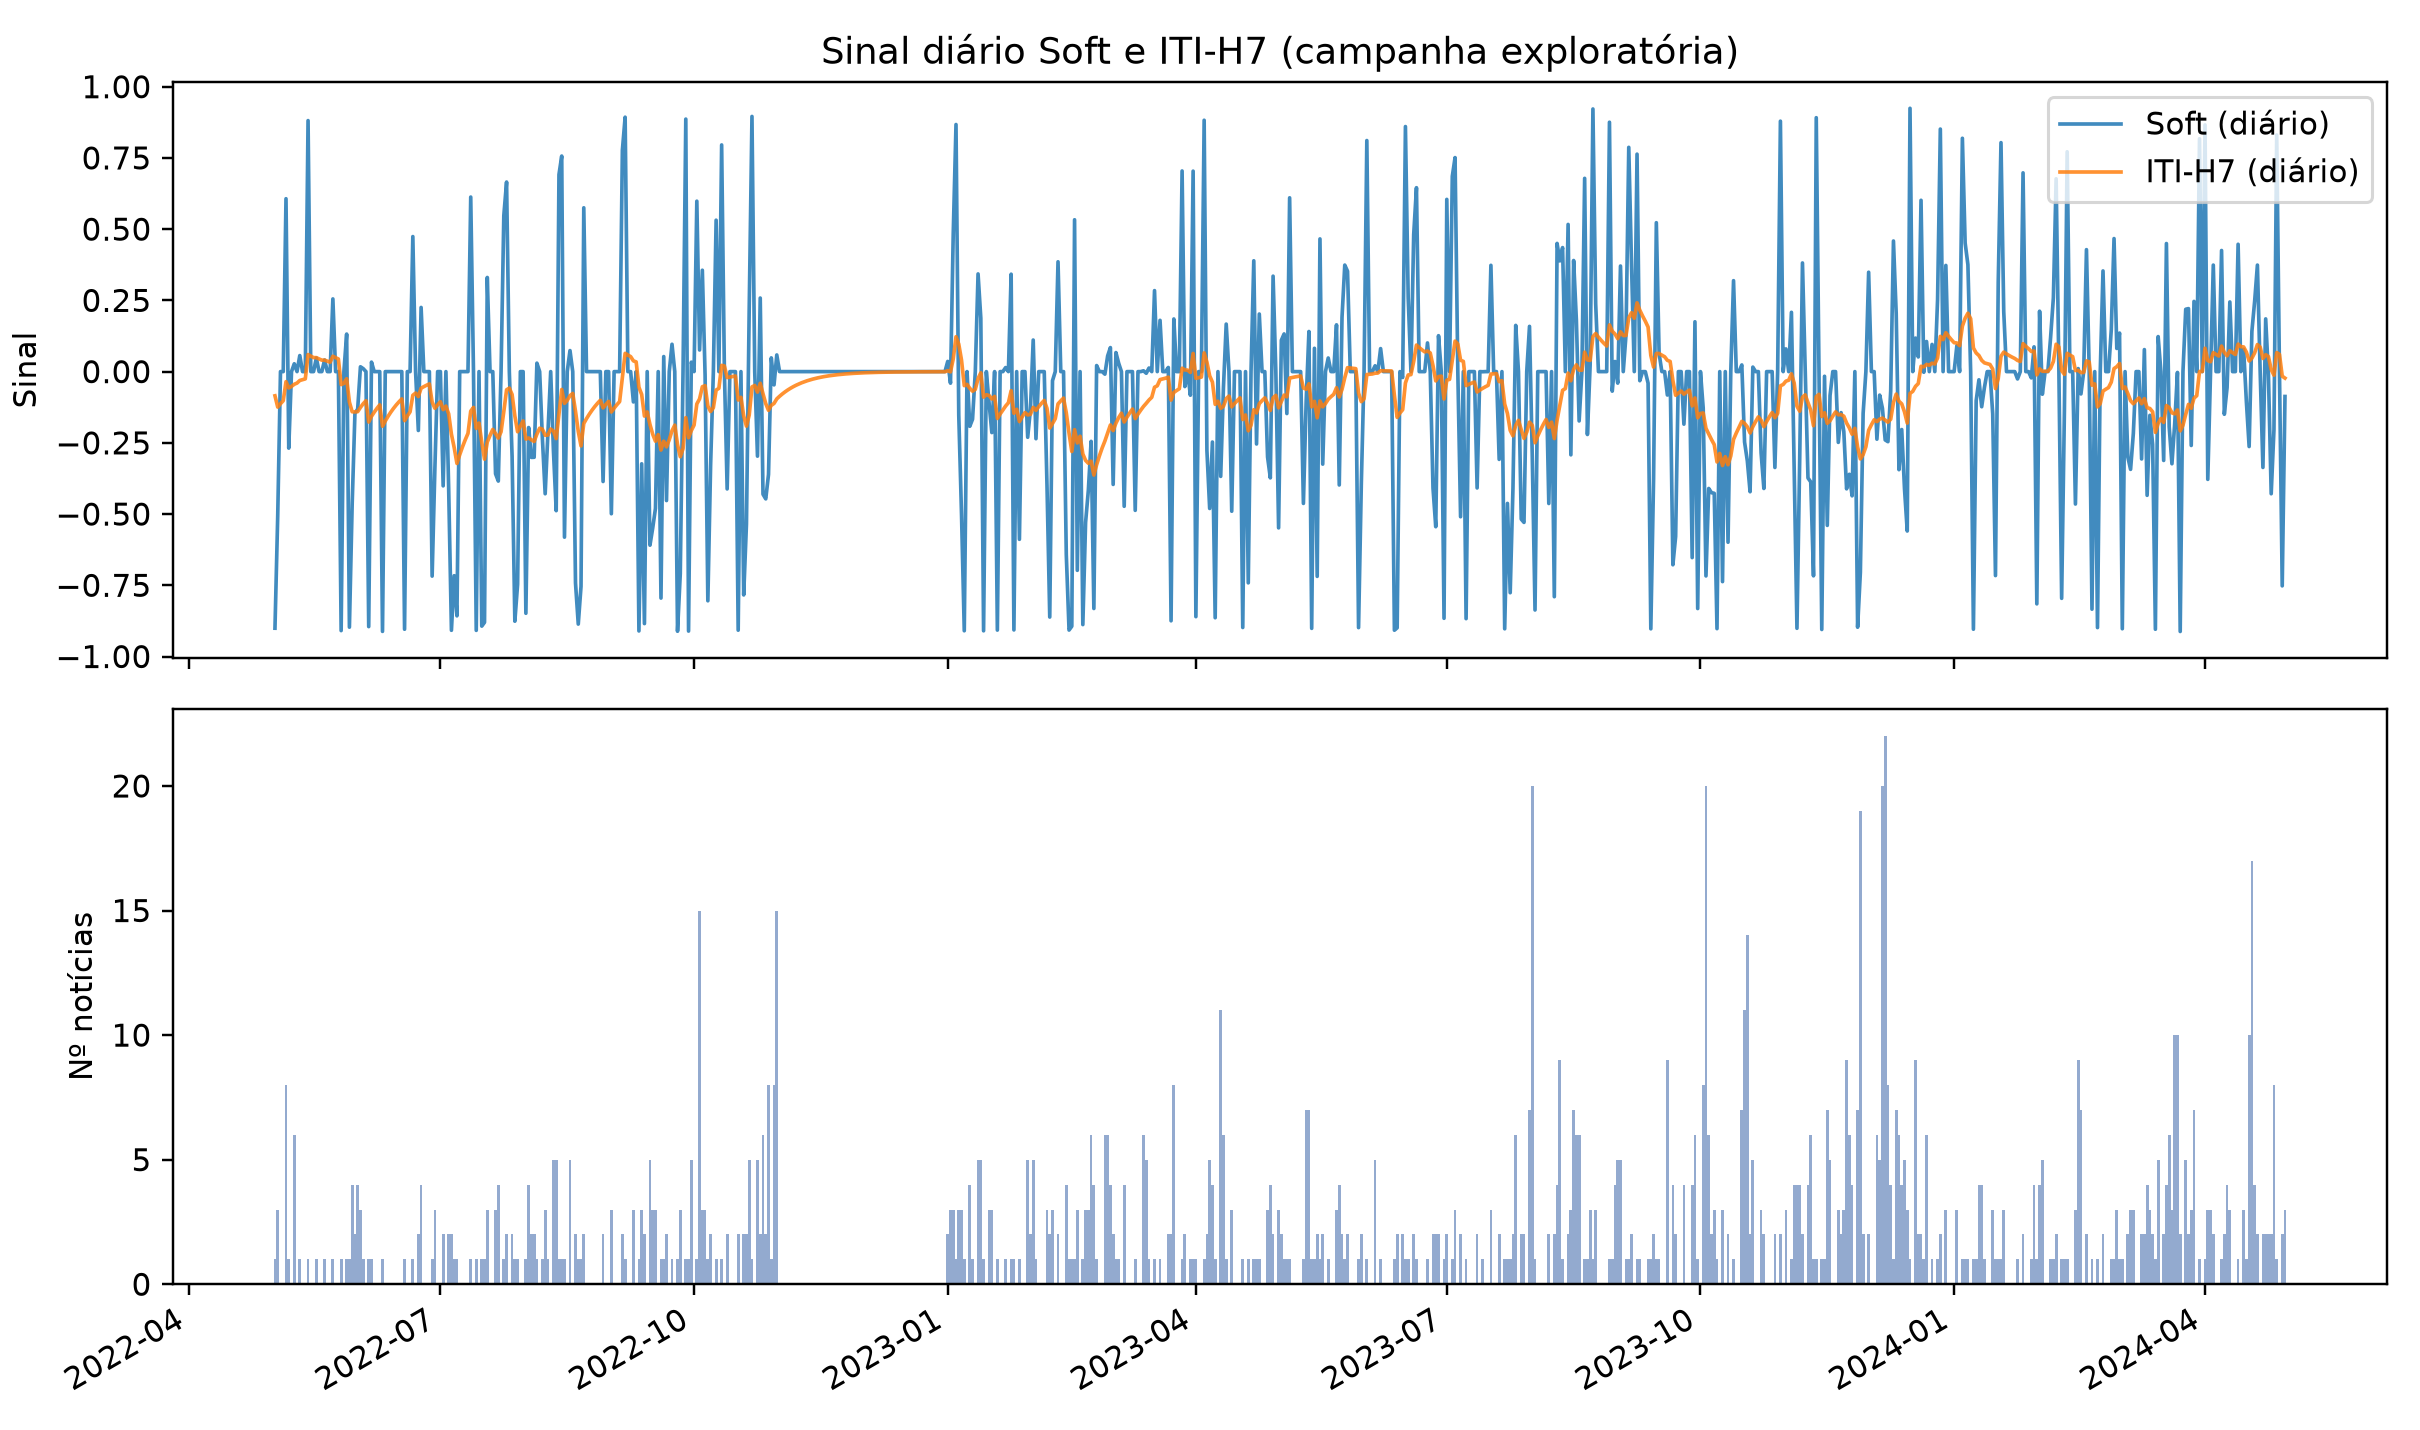
\includegraphics[width=0.92\linewidth]{generated/figures/iti_v2/figure_daily_signal.png}
\caption{Sinal diário sem memória (Soft), ITI-H7 e quantidade de notícias elegíveis.}
\label{fig:iti-campanha-1}
\par\smallskip
{\footnotesize\raggedright Fonte: elaboração própria, com dados da campanha de outubro de 2026.\par}
\end{figure}

A Figura~\ref{fig:iti-campanha-2} compara as séries com meias-vidas de dois, sete e quatorze dias calculadas sobre as mesmas probabilidades. Quanto maior a meia-vida, mais lentamente o estado anterior perde peso. Não há, contudo, motivo para interpretar a série mais suave como automaticamente mais adequada ao comportamento da ação.

\begin{figure}[H]
\centering
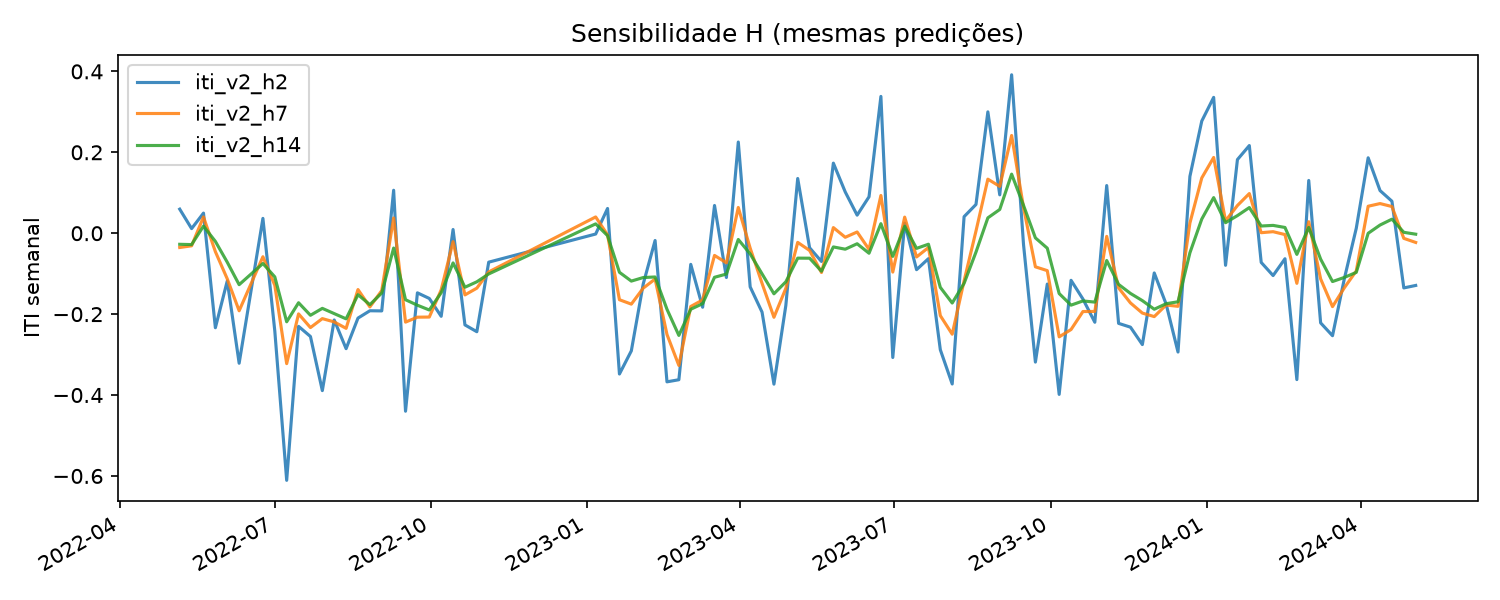
\includegraphics[width=0.88\linewidth]{generated/figures/iti_v2/figure_h_sensitivity.png}
\caption{Sensibilidade do ITI a diferentes meias-vidas: $H=2$, $H=7$ e $H=14$ dias civis.}
\label{fig:iti-campanha-2}
\par\smallskip
{\footnotesize\raggedright Fonte: elaboração própria, com dados da campanha de outubro de 2026.\par}
\end{figure}

A Figura~\ref{fig:iti-campanha-3} sintetiza as diferenças de correlação e os intervalos nominais dos contrastes secundários. A linha vertical em zero marca a ausência de diferença assinada. O ajuste de Holm se aplica aos valores $p$ da Tabela~\ref{tab:iti-secondary}, e não aos intervalos exibidos na figura.

\begin{figure}[H]
\centering
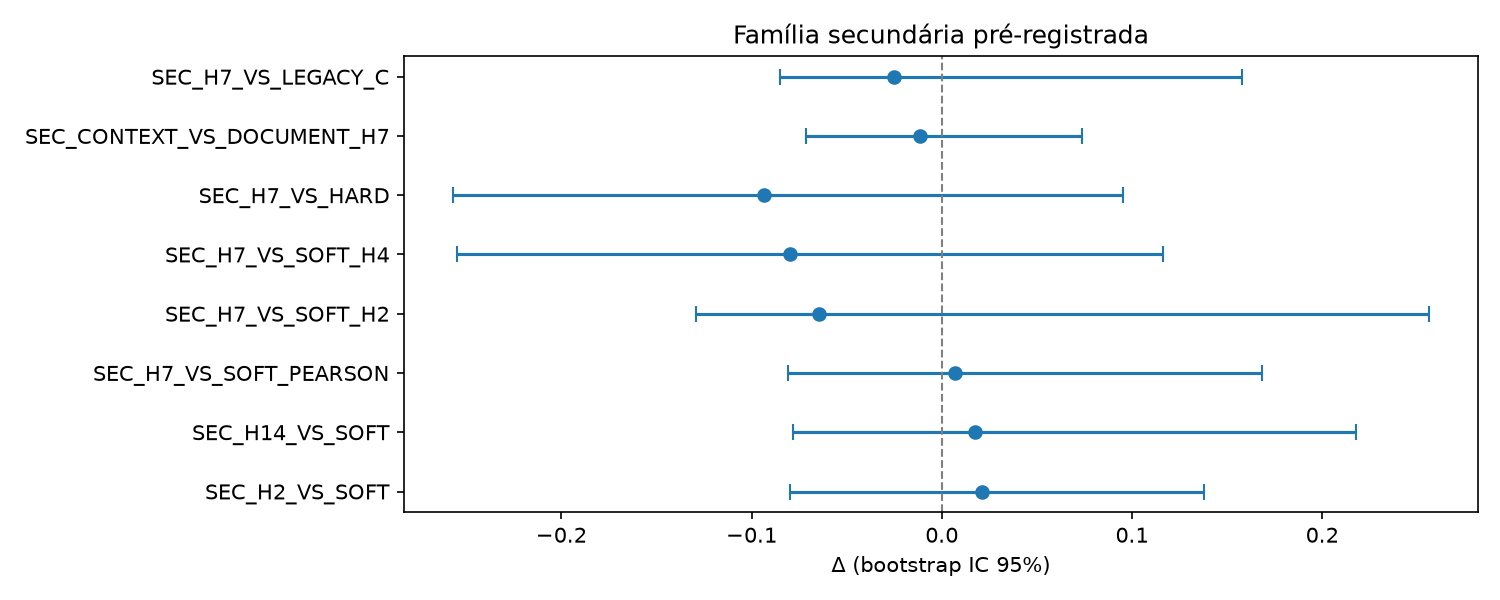
\includegraphics[width=0.88\linewidth]{generated/figures/iti_v2/figure_delta_intervals.png}
\caption{Diferenças de correlação dos contrastes secundários e intervalos bootstrap nominais de 95\%.}
\label{fig:iti-campanha-3}
\par\smallskip
{\footnotesize\raggedright Fonte: elaboração própria, com dados da campanha de outubro de 2026.\par}
\end{figure}
\FloatBarrier

\subsection{Interpretação do Soft e da média semanal}

A leitura do contraste principal depende da definição do Soft. Das 94 semanas comparadas, ele apresentou valor zero em 36, correspondentes a 38,3\% do conjunto. Em 33 dessas semanas, havia notícias em dias anteriores ao corte dentro da própria semana civil. Assim, Soft zero não significa necessariamente ausência de notícias durante toda a semana; pode significar somente que não houve matéria observada no dia específico em que o indicador foi amostrado.

Para examinar uma referência que também incorporasse vários dias, realizou-se uma comparação adicional entre o ITI-H7 e a média semanal dos sinais diários. No mesmo painel de 94 semanas, a diferença entre as correlações de Spearman foi de $-0{,}062$, com intervalo bootstrap nominal de 95\% $[-0{,}165;\,0{,}060]$ e valor $p$ exploratório de $0{,}340$. O intervalo inclui zero, de modo que a análise permanece inconclusiva.

Essa comparação adicional não integra a família de oito contrastes corrigida por Holm e não substitui retroativamente a hipótese principal. Ela torna explícita uma limitação do Soft pontual: o contraste inicial avalia memória em relação ao sinal do dia de corte, e não demonstra superioridade da memória exponencial sobre todas as estratégias que agregam notícias ao longo de uma semana.

\section{Discussão integrada e ameaças à validade}

Os resultados textuais e temporais precisam ser interpretados conjuntamente. A implementação permite calcular e comparar o ITI, mas a associação com retornos não corrige eventuais problemas nas probabilidades de sentimento. Em particular, a baixa concordância na avaliação baseada em título e corpo e a ausência de validação independente da entrada contextual impedem atribuir ao índice uma validade econômica que ainda não foi demonstrada.

A Tabela~\ref{tab:ameacas} reúne as principais ameaças observadas e as providências que podem reduzi-las na continuidade da pesquisa.

\begin{table}[htbp]
\centering
\caption{Ameaças à validade identificadas na etapa exploratória.}
\label{tab:ameacas}
\begin{tabularx}{\textwidth}{@{}P{0.19\textwidth}L L@{}}
\toprule
Dimensão & Limitação observada & Encaminhamento \\
\midrule
Construto & Discordâncias entre FinBERT e anotação do autor; entrada contextual ainda sem validação humana independente & Anotação independente e diagnóstico na mesma entrada do ITI \\
Desenho & Cobertura diária não comprovada em todo o corpus; informação de horários incompleta & Inventário auditável de fontes, datas e disponibilidade \\
Estatística & 94 semanas no contraste; intervalos amplos; testes exploratórios e múltiplas comparações & Novo período de avaliação com protocolo congelado \\
Externa & Estudo de caso da Sabesp, sem comparação equivalente entre empresas & Novos casos somente após documentar a cobertura e o alvo \\
Reprodução & Artefatos completos de execução não integralmente versionados no Git público & Preservar manifestos, checkpoint, preços e dados da campanha \\
\bottomrule
\end{tabularx}
\vspace{0.4em}
{\footnotesize Fonte: elaboração própria com base nas etapas e nos resultados da pesquisa.}
\end{table}

Em síntese, os experimentos mostram que o procedimento pode ser executado e examinado e identificam suas limitações mais importantes. Eles ainda não validam o ITI como indicador de impacto econômico das notícias sobre a Sabesp. O principal passo seguinte é verificar a qualidade das classificações que efetivamente entram no índice e repetir a avaliação temporal sob condições previamente definidas.
